\documentclass[aspectratio=169, 10pt]{beamer}

\usepackage{bm} % bold math
\usepackage{fontspec}
\usepackage{minted}
\usepackage{pgf-pie}
\usepackage{tikz}
\usepackage{graphicx}
\newcommand\sbullet[1][.5]{\mathbin{\vcenter{\hbox{\scalebox{#1}{$\bullet$}}}}}

% Custom commands and environments
\makeatletter
\newcommand\version[1]{\renewcommand\@version{#1}}
\newcommand\@version{}
\def\insertversion{\@version}

\newcommand\course[1]{\renewcommand\@course{#1}}
\newcommand\@course{}
\def\insertcourse{\@course}

\newcommand\coursetitle[1]{\renewcommand\@coursetitle{#1}}
\newcommand\@coursetitle{}
\def\insertcoursetitle{\@coursetitle}

\newcommand\lecturenumber[1]{\renewcommand\@lecturenumber{#1}}
\newcommand\@lecturenumber{}
\def\insertlecturenumber{\@lecturenumber}
\makeatother

\newcommand{\slidetitle}[1]{{\xbseries \large \structure{#1}} \bigskip}
\newcommand{\term}[1]{{\color{blue} #1}}
\newcommand{\leftspace}{\hspace{1em}}
\newcommand{\inlinearrow}{
  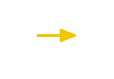
\begin{tikzpicture}[baseline]
    \node [anchor=base] (x) {};
    \draw [rawarrow] (x.mid west) -- ($(x.mid west) + (2em,0)$);
  \end{tikzpicture}
}

\newenvironment{slide}
{\begin{frame}[fragile,environment=slide]\vskip0pt plus 1filll}
{\vskip0pt plus 1filll\end{frame}}

% LaTeX

\setlength{\leftmargini}{1em}

% Common Information

\author{Talia Xu}
\course{COMPSCI 340}
\coursetitle{Operating Systems}
\date{2024 Semester 2}

% fontspec

\defaultfontfeatures{Ligatures=TeX}
% \setmainfont{Domine}
\setsansfont{Inter}[
  FontFace={ul}{n}{Font=*-Thin},
  FontFace={el}{n}{Font=*-ExtraLight},
  FontFace={l}{n}{Font=*-Light},
  FontFace={sb}{n}{Font=*-SemiBold},
  FontFace={eb}{n}{Font=*-ExtraBold},
  FontFace={xb}{n}{Font=*-Black},
]
\setmonofont[Contextuals=AlternateOff, Ligatures=TeXOff]{Iosevka}[
  FontFace={xb}{n}{Font=*-Heavy},
]

%% Font Weights

\DeclareRobustCommand{\ulseries}{\fontseries{ul}\selectfont}
\DeclareTextFontCommand{\textul}{\ulseries}
\DeclareRobustCommand{\elseries}{\fontseries{el}\selectfont}
\DeclareTextFontCommand{\textel}{\elseries}
\DeclareRobustCommand{\lseries}{\fontseries{l}\selectfont}
\DeclareTextFontCommand{\textl}{\lseries}
\DeclareRobustCommand{\sbseries}{\fontseries{sb}\selectfont}
\DeclareTextFontCommand{\textsb}{\sbseries}
\DeclareRobustCommand{\ebseries}{\fontseries{eb}\selectfont}
\DeclareTextFontCommand{\texteb}{\ebseries}
\DeclareRobustCommand{\xbseries}{\fontseries{xb}\selectfont}
\DeclareTextFontCommand{\textxb}{\xbseries}

% tikz

\usetikzlibrary{
  arrows,
  arrows.meta,
  automata,
  backgrounds,
  calc,
  decorations.pathreplacing,
  matrix,
  positioning,
  overlay-beamer-styles,
  shapes,
  shapes.multipart,
  tikzmark,
}

\tikzstyle{rawarrow} = [
  -{Latex[round]},
  line width=1pt,
  yellow,
  shorten >=3pt,
  shorten <=3pt,
  font=\small,
  text=black,
]

\tikzstyle{arrow} = [
  -{Latex[round]},
  line width=1pt,
  yellow,
  shorten >=3pt,
  shorten <=3pt,
  transform canvas={yshift=3pt},
  font=\small,
  text=black,
]

\newcommand{\tikzmarkcoord}[1]{([yshift=3pt]pic cs:#1)}

% minted

\setminted{style=eyolfson, fontsize=\small, escapeinside=||}
\setmintedinline{fontsize=\normalsize}

% hyperref

\hypersetup{colorlinks, urlcolor=blue}

% beamer
\setbeamersize{text margin left=16mm, text margin right=16mm}
\setbeamertemplate{itemize items}[circle]
\setbeamercolor{item}{fg=black}
\setbeamercolor{structure}{fg=darkblue}
\setbeamerfont{frametitle}{series=\bfseries, parent=structure}
\setbeamertemplate{navigation symbols}{}
\setbeamertemplate{headline}{}
\setbeamertemplate{footline}{
  \begin{tikzpicture}[
    remember picture,
    overlay,
    shift={(current page.south west)},
  ]
    \path [fill=gray] (144mm, 0) -- (160mm, 16mm) -- (160mm, 0);
    \node [inner sep=3.5mm, outer sep=0, text=black, anchor=base east,
           align=right, yshift=3.5mm]
          at (current page.south east) {\ttfamily \small \insertframenumber{}};
  \end{tikzpicture}
}
\setbeamertemplate{title page}{
  \begin{tikzpicture}[
    remember picture,
    overlay,
    shift={(current page.south west)},
    background rectangle/.style={fill=darkblue},
    show background rectangle,
  ]
    \node [anchor=center, align=center, text=white, text width=40mm, scale=3.2]
          at (\paperwidth / 2, \paperheight * 2 / 3)
          {\xbseries \inserttitle{}};
    \node [anchor=base west, align=left, inner sep=0, text=white, yshift=2.5mm]
          at (16mm, \paperheight / 3)
          {\insertdate{} \insertcourse{}: \insertcoursetitle{}};
    \node [anchor=base west, align=left, inner sep=0, text=white, yshift=-2.5mm]
          at (16mm, \paperheight / 3)
          {\insertauthor};
    \node [anchor=base east, align=right, inner sep=0, text=white, yshift=2.5mm]
          at (144mm, \paperheight / 3)
          {Lecture \insertlecturenumber{}};
    \node [anchor=base east, align=right, inner sep=0, text=white,
           yshift=-2.5mm]
          at (144mm, \paperheight / 3)
          {\ttfamily \insertversion{}};
    \node [align=center, anchor=south, inner sep=0, text=white, yshift=3.5mm]
          (license) at (\paperwidth / 2, 0)
          {\fontsize{7pt}{7pt}\selectfont This  work is licensed under a
           \href{http://creativecommons.org/licenses/by-sa/4.0/}
                {\color{lightblue} Creative Commons Attribution-ShareAlike 4.0
                 International License}};
  \end{tikzpicture}
}

% xcolor

%% Primary Colour

\definecolor{pantone655}{RGB}{0, 42, 92} % #002a5c
\colorlet{darkblue}{pantone655}

%% Secondary Colours

\definecolor{pantone633}{RGB}{0, 139, 176} % #008bb0
\colorlet{blue}{pantone633}

\definecolor{pantonewarmred}{RGB}{220, 70, 51} % #dc4633
\colorlet{red}{pantonewarmred}

\definecolor{pantone3285}{RGB}{0, 161, 137} % #00a189
\colorlet{cyan}{pantone3285}

\definecolor{pantone7722}{RGB}{13, 83, 77} % #0d534d
\colorlet{darkcyan}{pantone7722}

\definecolor{pantone376}{RGB}{141, 191, 46} % #8dbf2e
\colorlet{green}{pantone376}

\definecolor{pantone2613}{RGB}{109, 36, 122} % #6d247a
\colorlet{violet}{pantone2613}

\definecolor{pantone2985}{RGB}{111, 199, 234} % #6fc7ea
\colorlet{lightblue}{pantone2985}

\definecolor{pantone227}{RGB}{171, 19, 104} % #ab1368
\colorlet{magenta}{pantone227}

\definecolor{pantone7406}{RGB}{241, 197, 0} % #f1c500
\colorlet{yellow}{pantone7406}

%% Neutrals

\definecolor{pantonecoolgray2}{RGB}{208, 209, 201} % #d0d1c9
\colorlet{gray}{pantonecoolgray2}


\lecturenumber{1}
\title{Memory}
\version{1.0.0}

\begin{document}

\begin{frame}[plain, noframenumbering]
    \titlepage
\end{frame}

\begin{slide}

    \slidetitle{Static Allocation is the Simplest Strategy}

    Create a fixed size allocation in your program

    \leftspace{}e.g. \mintinline{c}{char buffer[4096];}
    \medskip

    When the program loads, the kernel sets aside that memory
    for you
    \medskip

    That memory exists as long as your process does, no need to free

\end{slide}

\begin{slide}

    \slidetitle{Dynamic Allocation is Often Required}

    You may only conditionally require memory

    \leftspace{}Static allocations are sometimes wasteful
    \medskip

    You may not know the size of the allocation

    \leftspace{}Static allocations need to account for the maximum size
    \medskip

    Where do you allocate memory?

    \leftspace{}You can either allocate on the stack or on the heap

\end{slide}

\begin{slide}

    \slidetitle{Stack Allocation is Mostly Done for You in C}

    Think of normal variables

    \leftspace{}e.g. \mintinline{c}{int x;}
    \medskip

    The compiler internally inserts \mintinline{c}{alloca} calls

    \leftspace{}e.g. \mintinline{c}{int *px = (int*) alloca(4);}
    \medskip

    Whenever the function that called \mintinline{c}{alloca} returns, it
    frees all the memory

    \leftspace{}This just restores the previous stack pointer
    \medskip

    This won't work if you try to use the memory after returning

\end{slide}

\begin{slide}

    \slidetitle{You've Used Dynamic Allocation Before}

    These are the \mintinline{c}{malloc} family of functions
    \medskip

    The most flexible way to use memory, but is also the most difficult to get
    right
    \medskip

    You have to properly handle your memory lifetimes, and \mintinline{c}{free}
    exactly once
    \medskip

    Also, there's a new concern --- fragmentation

\end{slide}

\begin{slide}

    \slidetitle{Fragmentation is a Unique Issue for Dynamic Allocation}

    You allocate memory in different sized contiguous blocks

    \leftspace{}Compaction is not possible and every allocation decision is
    permanent
    \medskip

    A fragment is a small contiguous block of memory that cannot handle an
    allocation

    \leftspace{}You can think of it as a ``hole'' in memory, wasting space
    \medskip

    There are 3 requirements for fragmentation
    \begin{enumerate}
        \item Different allocation lifetimes
        \item Different allocation sizes
        \item Inability to relocate previous allocations  
    \end{enumerate}

\end{slide}

\begin{slide}
    
    \slidetitle{There's Internal and External Fragmentation}

    External fragmentation occurs when you allocate different sized blocks

    \leftspace{}There's no room for an allocation between the blocks

    \begin{center}
    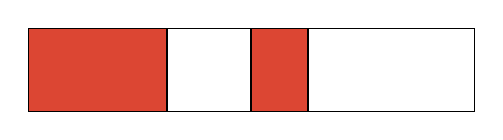
\begin{tikzpicture}[node distance=0mm and 0mm]
      \node[draw,rectangle,minimum width=50,minimum height=30,fill=red]
        (a0) {};
      \node[draw,rectangle,minimum width=30,minimum height=30]
        (a1) [right=of a0] {};
      \node[draw,rectangle,minimum width=20,minimum height=30,fill=red]
        (a2) [right=of a1] {};
      \node[draw,rectangle,minimum width=60,minimum height=30]
        (a3) [right=of a2] {};
    \end{tikzpicture}
    \end{center}

    Internal fragmentation occurs when you allocate fixed sized blocks

    \leftspace{}There's wasted space within a block

    \begin{center}
    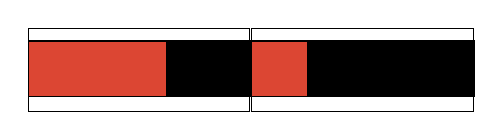
\begin{tikzpicture}[node distance=0mm and 0mm]
      \node[draw,rectangle,minimum width=50,minimum height=20,fill=red]
        (a0) {};
      \node[draw,rectangle,minimum width=30,minimum height=20,fill=black]
        (a1) [right=of a0] {};
      \node[draw,rectangle,minimum width=20,minimum height=20,fill=red]
        (a2) [right=of a1] {};
      \node[draw,rectangle,minimum width=60,minimum height=20,fill=black]
        (a3) [right=of a2] {};
      \node[draw,rectangle,minimum width=80,minimum height=30,xshift=15,yshift=25]
        [below=of a0] {};
      \node[draw,rectangle,minimum width=80,minimum height=30,xshift=30,yshift=25]
        [below=of a2] {};
    \end{tikzpicture}
    \end{center}

    \begin{flushright}
      Credit: \href{https://git.scc.kit.edu/uurqi/os-tutorium}{Daniel Ritz}
    \end{flushright}

\end{slide}

\begin{slide}

    \slidetitle{We Want to Minimize Fragmentation}

    Fragmentation is just wasted space, which we should prevent
    \medskip

    We want to reduce the number of ``holes'' between blocks of memory

    \leftspace{}If we have holes, we'd like to keep them as large as possible
    \medskip

    Our goal is to keep allocating memory without wasting space

\end{slide}

\begin{slide}

    \slidetitle{Allocator Implementations Usually Use a Free List}

    They keep track of free blocks of memory by chaining them together

    \leftspace{}Implemented with a linked list
    \medskip

    We need to be able to handle a request of any size
    \medskip

    For allocation, we choose a block large enough for the request

    \leftspace{}Remove it from the free list
    \medskip

    For deallocation, we add the block back to the free list

    \leftspace{}If it's adjacent to another free block, we can merge them

\end{slide}

\begin{slide}

    \slidetitle{There are 3 General Heap Allocation Strategies}

    Best fit: choose the smallest block that can satisfy the request

    \leftspace{}Needs to search through the whole list (unless there's an
    exact match)
    \medskip

    Worst fit: choose largest block (most leftover space)

    \leftspace{}Also has to search through the list
    \medskip
    
    First fit: choose first block that can satisfy request
\end{slide}

\begin{slide}
    
    \slidetitle{Allocating Using Best Fit (1)}

    Note that blocks with a blank background and a number are free
    \medskip

    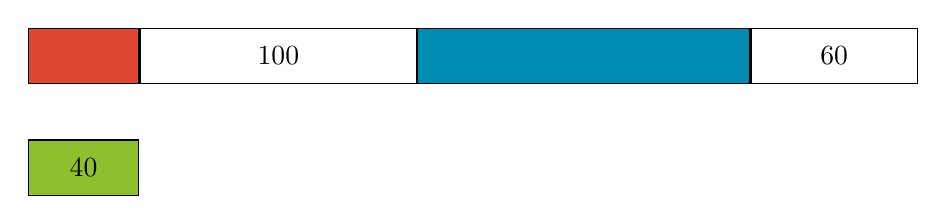
\begin{tikzpicture}[node distance=0mm and 0mm]
      \node[draw,rectangle,minimum width=40,minimum height=20,fill=pantonewarmred]
        (a0) {};
      \node[draw,rectangle,minimum width=100,minimum height=20]    (a1)  [right=of a0]      {100};
      \node[draw,rectangle,minimum width=120,minimum height=20,fill=pantone633]    (a2) [right=of a1]       {};
      \node[draw,rectangle,minimum width=60,minimum height=20]    (a3)    [right=of a2]    {60};

      \node[draw,rectangle,minimum width=40,minimum height=20,yshift=-20,fill=pantone376]
        [below=of a0] {40};
    \end{tikzpicture}

    Where do we allocate this block?
\end{slide}

\begin{slide}
    
    \slidetitle{Allocating Using Best Fit (2)}

    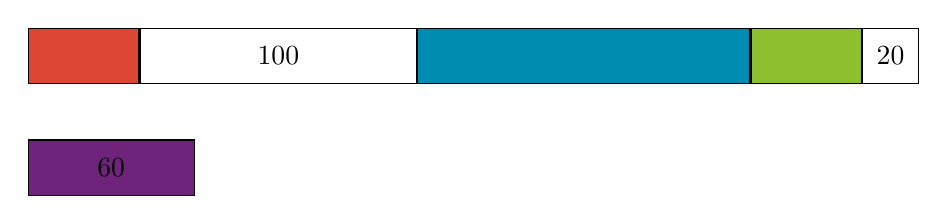
\begin{tikzpicture}[node distance=0mm and 0mm]
            
      \node[draw,rectangle,minimum width=40,minimum height=20,fill=pantonewarmred]    (a0)        {};
      \node[draw,rectangle,minimum width=100,minimum height=20]    (a1)  [right=of a0]      {100};
      \node[draw,rectangle,minimum width=120,minimum height=20,fill=pantone633]    (a2) [right=of a1]       {};
      \node[draw,rectangle,minimum width=40,minimum height=20,fill=pantone376]    (a3)    [right=of a2]    {};
      \node[draw,rectangle,minimum width=20,minimum height=20]    (a4)    [right=of a3]    {20};

      \node[draw,rectangle,minimum width=60,minimum height=20,yshift=-20,xshift=10,fill=pantone2613] [below=of a0] {60};

    \end{tikzpicture}

    Where do we allocate this block?

\end{slide}

\begin{slide}

    \slidetitle{Allocating Using Best Fit (3)}

    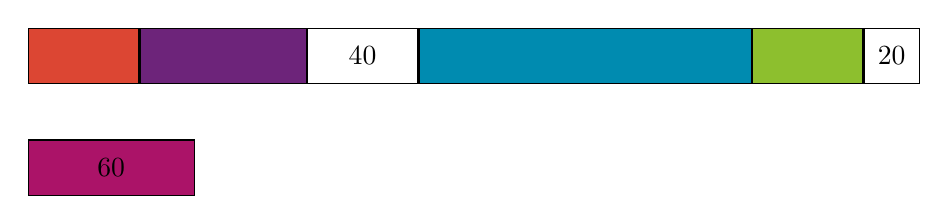
\begin{tikzpicture}[node distance=0mm and 0mm]
      \node[draw,rectangle,minimum width=40,minimum height=20,fill=pantonewarmred]    (a0)        {};
      \node[draw,rectangle,minimum width=60,minimum height=20,fill=pantone2613]    (a1)  [right=of a0]      {};
      \node[draw,rectangle,minimum width=40,minimum height=20]    (a2)  [right=of a1]      {40};
      \node[draw,rectangle,minimum width=120,minimum height=20,fill=pantone633]    (a3) [right=of a2]       {};
      \node[draw,rectangle,minimum width=40,minimum height=20,fill=pantone376]    (a4)    [right=of a3]    {};
      \node[draw,rectangle,minimum width=20,minimum height=20]    (a5)    [right=of a4]    {20};

      \node[draw,rectangle,minimum width=60,minimum height=20,yshift=-20,xshift=10,fill=pantone227] [below=of a0] {60};
    \end{tikzpicture}

    The next block does not fit anywhere

\end{slide}

\begin{slide}
    
    \slidetitle{Allocating Using Worst Fit (1)}

    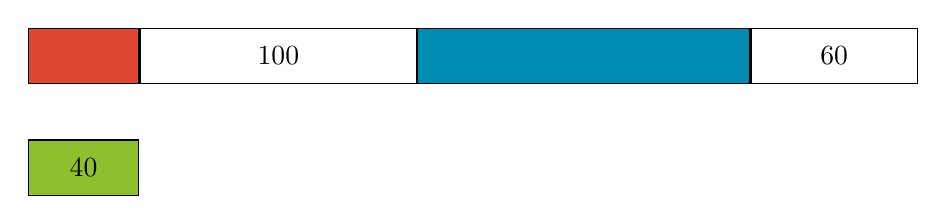
\begin{tikzpicture}[node distance=0mm and 0mm]
        \node[draw,rectangle,minimum width=40,minimum height=20,fill=pantonewarmred]    (a0)        {};
        \node[draw,rectangle,minimum width=100,minimum height=20]    (a1)  [right=of a0]      {100};
        \node[draw,rectangle,minimum width=120,minimum height=20,fill=pantone633]    (a2) [right=of a1]       {};
        \node[draw,rectangle,minimum width=60,minimum height=20]    (a3)    [right=of a2]    {60};

        \node[draw,rectangle,minimum width=40,minimum height=20,yshift=-20,fill=pantone376] [below=of a0] {40};
    \end{tikzpicture}

    Where do we allocate this block?

\end{slide}

\begin{slide}
    
    \slidetitle{Allocating Using Worst Fit (2)}

    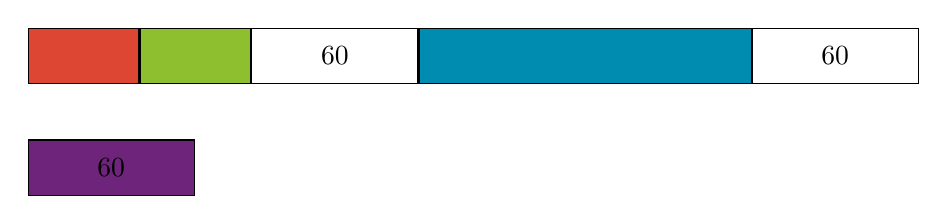
\begin{tikzpicture}[node distance=0mm and 0mm]
        \node[draw,rectangle,minimum width=40,minimum height=20,fill=pantonewarmred]    (a0)        {};
        \node[draw,rectangle,minimum width=40,minimum height=20,fill=pantone376]    (a1)  [right=of a0]      {};
        \node[draw,rectangle,minimum width=60,minimum height=20]    (a2)    [right=of a1]    {60};
        \node[draw,rectangle,minimum width=120,minimum height=20,fill=pantone633]    (a3) [right=of a2]       {};
        \node[draw,rectangle,minimum width=60,minimum height=20]    (a4)    [right=of a3]    {60};

        \node[draw,rectangle,minimum width=60,minimum height=20,yshift=-20,xshift=10,fill=pantone2613] [below=of a0] {60};
    \end{tikzpicture}

    Where do we allocate this block?

\end{slide}

\begin{slide}
    
    \slidetitle{Allocating Using Worst Fit (3)}

    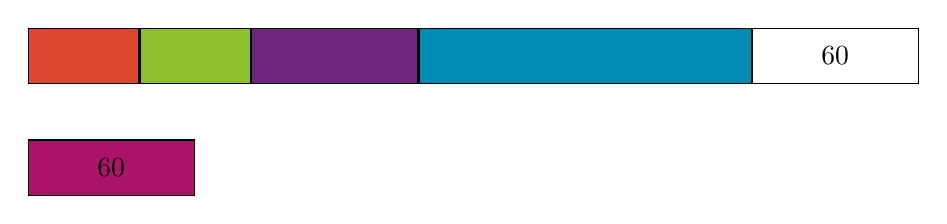
\begin{tikzpicture}[node distance=0mm and 0mm]
        \node[draw,rectangle,minimum width=40,minimum height=20,fill=pantonewarmred]    (a0)        {};
        \node[draw,rectangle,minimum width=40,minimum height=20,fill=pantone376]    (a1)  [right=of a0]      {};
        \node[draw,rectangle,minimum width=60,minimum height=20,fill=pantone2613]    (a2)    [right=of a1]    {};
        \node[draw,rectangle,minimum width=120,minimum height=20,fill=pantone633]    (a3) [right=of a2]       {};
        \node[draw,rectangle,minimum width=60,minimum height=20]    (a4)    [right=of a3]    {60};

        \node[draw,rectangle,minimum width=60,minimum height=20,yshift=-20,xshift=10,fill=pantone227] [below=of a0] {60};
    \end{tikzpicture}

    Next block fits exactly in remaining space

\end{slide}

\begin{slide}

    \slidetitle{Best Fit and Worst Fit are Both Slow}

    Best fit: tends to leave very large holes and very small holes

    \leftspace{}Small holes may be useless
    \medskip

    Worst fit: simulation says it's the worst in terms of storage utilization
    \medskip

    First fit: tends to leave ``average'' size holes

\end{slide}

\begin{slide}

    \slidetitle{The Kernel Has To Implement It's Own Memory Allocations}

    The concepts are the same for user space memory allocation

    (the kernel just gives them more contiguous virtual memory pages):

    \begin{itemize}
      \item There's static and dynamic allocations
      \item For dynamic allocations, fragmentation is a big concern
      \item Dynamic allocation returns blocks of memory
        \begin{itemize}
          \item Fragmentation between blocks is external
          \item Fragmentation within a blocks is internal
        \end{itemize}
      \item There's 3 general allocation strategies for different sized
            allocations
        \begin{itemize}
          \item Best fit
          \item Worst fit
          \item First fit
        \end{itemize}
    \end{itemize}

\end{slide}
  
\end{document}
